\documentclass[11pt,fleqn,a4paper,]{LegrandOrangeBook}
\addbibresource{sample.bib} % Bibliography file
\definecolor{ocre}{RGB}{243, 102, 25} 
\chapterimage{orange1.jpg} 
\chapterspaceabove{6.5cm}
\chapterspacebelow{6.75cm} 
%\begin{theorem}[Name of the theorem]
%\begin{exercise}
%\begin{example}[Example name]
%\begin{definition}[Definition name]
%\begin{corollary}[Corollary name]
%\begin{remark}
%\begin{proposition}[Proposition name]
%\begin{problem}
%\begin{vocabulary}[Word]
%\begin{notation}
%----------------------------------------------------------------------------------------
\begin{document}
%----------------------------------------------------------------------------------------
%----------------------------------------------------------------------------------------
%Lineas
%----------------------------------------------------------------------------------------
\section{Leyes de maxwell}\index{Leyes de maxwell}
Se presentan las ecuaciones de Maxwell en la tabla \ref{tab:maxwell}.
\begin{table}[]
\begin{tabular}{|l|m{0.3\linewidth}|l|}
\hline
\rowcolor[HTML]{FFFC9E} 
Forma diferencial                                  & Forma integral                                                                 & Remark                     \\ \hline
$\nabla\cdot \textbf{D}=\rho_v$                             & \begin{displaymath}
\oint_S\textbf{D}\cdot d\textbf{S}=\int_v\rho_vdv                                 \end{displaymath} & Ley de Gauss               \\ \hline
$\nabla\cdot \textbf{B}=0$                                  & \begin{displaymath}
\oint_S\textbf{B}\cdot d\textbf{S}=0
\end{displaymath}                                                           & No existencia de monopolos \\ \hline
$\nabla\times \textbf{E}=-\frac{\partial \textbf{B}}{\partial t}$    & \begin{displaymath}
\oint_L\textbf{E}\cdot dl=-\frac{\partial}{\partial t}\int_S\textbf{B}\cdot dS
\end{displaymath}                  & Ley de Faraday             \\ \hline
$\nabla\times \textbf{H}=\textbf{J} + \frac{\partial \textbf{D}}{\partial t}$ & \begin{displaymath}
\oint_L\textbf{H}\cdot dl=\int_S\left(\textbf{J} + \frac{\partial \textbf{D}}{\partial t}\right)\cdot d\textbf{S}
\end{displaymath} & Ley de circuitos de Ampere \\ \hline
\end{tabular}
\caption{Leyes de Maxwell}
\label{tab:maxwell}
\end{table}
Donde es necesario recordar el operador DEL (\ref{subsec:DEL})
\begin{itemize}
\item El gradiente de un escalar V: $\nabla$V
\item La divergencia de un vector A: $\nabla\cdot$A
\item La rotacional de un vector A: $\nabla\times$A
\item El Laplaciano de un escalar V: $\nabla^2$V
\end{itemize}
Además se tienen ecuaciones auxiliares:
\begin{subequations}
\begin{align}
\intertext{Relación entre la Densidad de Campo Eléctrico y la Intensidad de Campo Eléctrico.}
\textbf{D}&= \epsilon \textbf{E}\\
\intertext{Relación entre la Densidad de Campo Magnético y la Intensidad de Campo Magnético.}
\textbf{B}&=\mu\textbf{H}\\
\intertext{Densidad de Corriente de conducción.}
\textbf{J}&=\sigma\textbf{E}\\
\intertext{Densidad de Corriente de convección en función de la densidad de carga volumétrica.}
\textbf{J}&=\rho_v\textbf{v}
\end{align}
\end{subequations}
Hay ligeras modificaciones si son para conductores malos (aislantes):
\begin{subequations}
\begin{align}
\textbf{D}&= \epsilon \textbf{E} + P\\
\textbf{B}&=\mu(\textbf{H} + M)
\end{align}
\end{subequations}
Donde P es el campo de polarización y M es el campo de magnetización, cuando el dieléctrico es lineal se tiene:
\begin{align*}
&P=\chi_e\epsilon_0\textbf{E} &M=\chi_m\textbf{H}
\end{align*}
%\section{Modelo electromagnético y las leyes de Maxwell}
%----------------------------------------------------------------------------------------
%Internetworking
%----------------------------------------------------------------------------------------
\section{Satélites}\index{Satélites}
En su forma más simple, podemos considerar un satélite de comunicaciones como un enorme repetidor de microondas en el cielo que contiene varios transpondedores, cada uno de los cuales escucha en cierta porción del espectro, amplifica la señal entrante y después la retransmite en otra frecuencia para evitar interferencia con la señal entrante. Este modo de operación se llama \textbf{tubo doblado}. De acuerdo con la ley de Kepler, el periodo orbital de un satélite varía según el radio de la órbita a la 3/2 potencia. Entre más alto esté el satélite, mayor será el periodo. El periodo de un satélite es importante, pero no es la única razón para determinar en dónde colocarlo.\\
Otra cuestión es la presencia de los cinturones de Van Allen: capas de partículas altamente cargadas, atrapadas por el campo magnético de la Tierra. Cualquier satélite que volara dentro de los cinturones quedaría destruido casi al instante debido a las partículas (Fig. \ref{fig: satelites prop}).
\begin{figure}[]
\centering
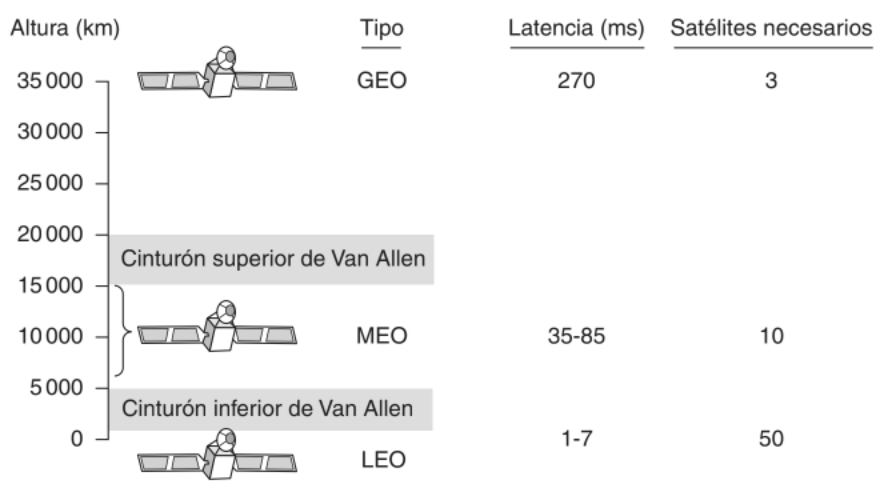
\includegraphics[width=\linewidth]{IN1/IN21.png}
\caption{Satélites de comunicaciones y algunas de sus propiedades, incluyendo la altitud sobre la Tierra, el tiempo de retardo de viaje redondo y la cantidad de satélites necesarios para una cobertura global.}
\label{fig: satelites prop}
\end{figure}
\subsection{Satélites geoestacionarios-GEO}
Actualmente los satélites se encuentran a no menos de 2° de distancia en el plano ecuatorial con el fin de evitar interferencias. Teniendo en cuenta el máximo de satélites es de 360°/2°=180 satélites, sin embargo cada transponedor puede usar múltiple frecuencias y polarizaciones para ampliar su ancho de banda.\\
Los satélites suelen tener una vida de 10 años aprox., tiempo en el cual se gasta el combustible usado para que los motores puedan realizar \textbf{control de posición orbital}, proceso por el cual un satélite se tiene que auto-calibrar en su órbita debido a que la gravedad solar, lunar y planetaria los saca de su órbita. La energía suficiente para que funcione un satélite viene de sus paneles solares; cuando un de estos este fuera de servicio, su órbita se deteriora sola quedando flotando en el vacío, se debe desactivar y esperar su destrucción aunque rara vez los satélite caen la tierra, (5 toneladas) impactan en forma de pedazos.\\
La ITU tambien a asignado bandas de frecuencias especificas a los usuarios de satélites (Tabla \ref{tab: banda sat}). Existen dos rangos de frecuencia asignadas a las bandas: enlace descendente (proveniente del satélite) y ascendente (hacia el satélite)
\begin{table}[]
\begin{tabular}{lllll}
\rowcolor[HTML]{FFCE93} 
Banda & Enlace descendente & Enlace ascendente & Ancho de Banda & Problemas                                                              \\
L     & 1.5 GHz            & 1.6 GHz           & 15 MHz         & \begin{tabular}[c]{@{}l@{}}Bajo ancho de banda\\ Saturada\end{tabular} \\
S     & .1.9 GHz           & 2.2 GHz           & 70 MHz         & \begin{tabular}[c]{@{}l@{}}Bajo ancho de banda\\ Saturada\end{tabular} \\
C     & .4.0 GHz           & 6.0 GHz           & 500 MHz        & Interferencia terrestre                                                \\
Ku    & 11 GHz             & 14 GHz            & 500 MHz        & Lluvia                                                                 \\
Ka    & 20 GHz             & 30 GHz            & 3500 MHz       & Lluvia, costo alto.                                                   
\end{tabular}
\caption{Principales bandas de satélites.}
\label{tab: banda sat}
\end{table}
Las que aún no están saturadas son las bandas K superior e inferior, a sus frecuencias más altas permite que los satélites estén a 1° de separación aunque la debilidad es el agua, ya que absorbe estas microondas cortas, aunque puede ser pronosticado para usar más estaciones terrestres a costa de usar más recursos. La K superior es usada para el tráfico comercial, militares y gubernamentales de satélites pero el equipo es costoso.\\
Lo que se usa comunmente aqui son las ``estaciones" \textbf{VSAT}, microestaciones que no son posibles de enviar datos(al menos por si solas) a otras microestaciones debido a su velocidad de subida de 1Mbps pero siendo su bajada de varios Mbps, es por ello que necesitas un antena más grande llamada \textbf{HUB} (Fig. \ref{fig: vsat hub}), que recibe la señal, la amplifica para enviarla a su destino aunque tiene a desventaja un mayor retardo.
\begin{figure}[H]
\centering
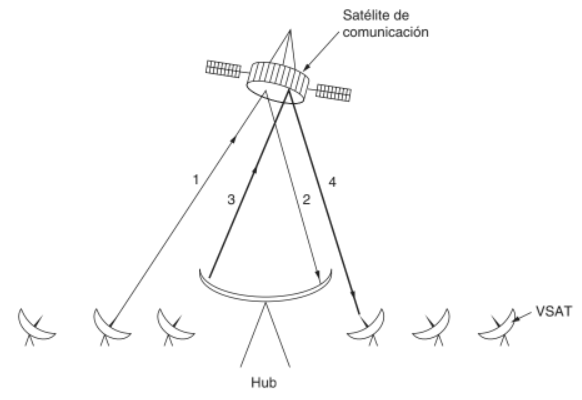
\includegraphics[width=0.5\linewidth]{IN1/IN22.png}
\caption{VSAT usando un HUB.}
\label{fig: vsat hub}
\end{figure}
\subsection{Satélites de órbita media-MEO}
Situadas entre los cinturones de Van Allen (Fig. \ref{fig: satelites prop}), tardan 6 horas en dar la vuelta a la tierra, por lo que hay que estar rastreandolos a medida que se mueven por el cielo, al estar a menor altura que los GEO producen una huella pequeña en la tierra y no requieren poderosos transmisores, actualmente estos se usan para sistemas de navegación en vez de telecomunicaciones, por ejemplo el GPS, posee 30 satélites que giran a una distancia de 20 200Km.
\subsection{Satélites de órbita terrestre baja-LEO}
Aún por debajo de los MEO, se encuentran los LEO, de gran movimiento pero de gran número de unidades para tener un sistema completo, no necesitas mucha potencia y son económicos.\\
\textbf{Iridium}\\
Desarrollados por Motorola, paso de ser 77 satélites lanzados inicialmente a 66,  con la premisa que tan pronto como un satélite quedará fuera del campo de visión de un usuario, otro ocuparía su lugar. Ofrece servicios de voz, datos, radiolocalización, fax y navegación en tierra, aire y mar, por medio de dispositivos portátiles que se comunican de manera directa con los satélites Iridium. Tiene clientes como entidades gubernamentales, militares marítimas, aviación y personas que viajan a lugares donde no hay infraestructura de telecomunicaciones (desiertos, montañas, el Polo Sur y algunos países del Tercer Mundo).\\
Estos satélites estan a una altura de 750 Km en orbitas polares circulares, separados a 32° de latitud cada anillo (Fig. \ref{fig: iridium}). Cada satélite tiene un máximo de 48 celdas (haces puntuales) y una capacidad de 3 840 canales, algunos de los cuales se utilizan para radiolocalización y navegación, mientras que otros se utilizan para datos y voz.
\begin{figure}[]
\centering
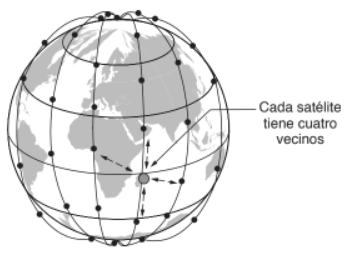
\includegraphics[width=\linewidth]{IN1/IN23.png}
\caption{Los satélites Iridium forman un seis collares al rededor de la Tierra.}
\label{fig: iridium}
\end{figure}
La comunicación de Iridium se realiza por el espacio (Fig. \ref{fig: iridium-global}.a), los satélites transmiten la llamada a través de la rejilla y la envía de nuevo a la tierra cuando llega a su destino. Una alternativa para este diseño es \textbf{Globalstar}, 48 satélites LEO que utilizan el concepto de \textbf{tubo doblado}, con el mismo ejemplo de la llamada, la llamada sale del usuario en el polo norte, se envía a al receptor terrestre más cercano, se hace el envió por tierra y se entrega al satelite más cercano al receptor (Fig. \ref{fig: iridium-global}.b), es obvio que la complejidad es menor pues estando en la tierra la conexión se pueden solucionar errores o hacer modificaciones más rápido. Además, el uso de antenas grandes en la estación en tierra que pueden enviar una señal potente y recibir una débil significa que se pueden utilizar teléfonos de baja potencia. Después de todo, el teléfono sólo emite unos cuantos miliwatts de potencia, de modo que la señal que llega a la estación en tierra es muy débil, aún después de que el satélite la haya amplificado.
\begin{figure}[]
\centering
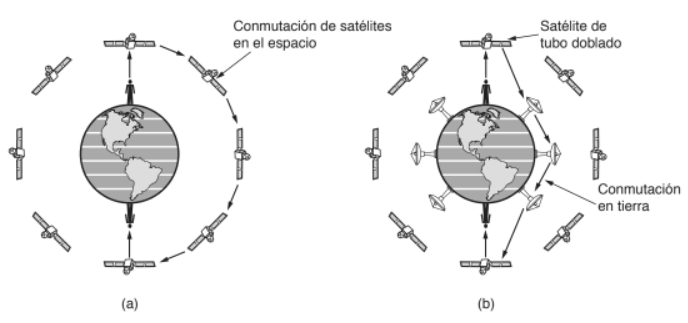
\includegraphics[width=\linewidth]{IN1/IN24.png}
\caption{(a) Transmisión en el espacio. (b) Transmisión en la tierra.}
\label{fig: iridium-global}
\end{figure}
\begin{proposition}[DNS: Resolución de IP a traves de nombres de maquina.]
Existe dos formas: \textbf{iterativamente}:
\begin{center}
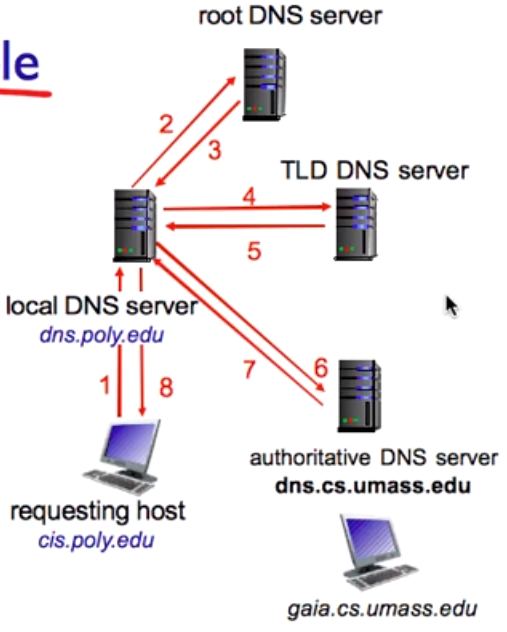
\includegraphics[scale=0.3]{IN1/IN19}
\end{center}
Si vemos las flechas numeradas. Primero el cliente consulta a su DNS local, asumiendo que no lo tienen, el DNS local  le preguntará al root DNS server (uno a nivel mundial), si no lo sabe lo redirecciona al TLD (Top level domain) DNS server que es el que tiene ese nombre. Asi el local DNS le preguntará al TLD DNS server. De no saberlo, el TLD lo dará la dirección del Authoritative DNS server. Y cuando lo tenga este le dará el IP de la PC con el nombre.\\
La segunda forma es \textbf{Recursiva}:
\begin{center}
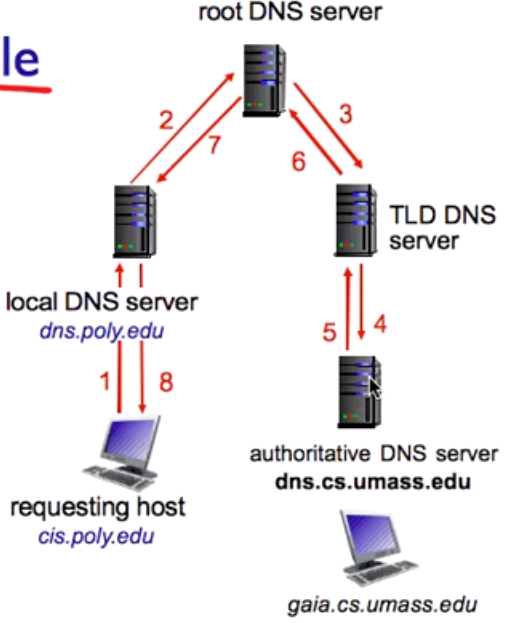
\includegraphics[scale=0.3]{IN1/IN20.png}
\end{center}
Busca en cada DNS server, creando una red ``directa'' entre ambos PC, lo malo de esta manera es que sobrecarga cada nivel, es por eso que las direcciones se guardan en un archivo caché, que se actualizarán cada cierto tiempo, el problema es que si cambias un nombre no funcionará la conexión hasta que se actualicé esta caché.
\end{proposition}
\section{Modulación digital y multiplexión}\index{Modulación digital y multiplexión}
\subsection{Transmisión Pasa-banda}
Incluso para los cables, es útil colocar una señal en una banda de frecuencias \textbf{específica} para dejar que \textbf{coexistan} distintos tipos de señales en el canal. A este tipo de transmisión se le conoce como \textbf{transmisión pasa-banda}, debido a que se utiliza una banda arbitraria de frecuencias para pasar la señal. Los valores absolutos de la frecuencia \textbf{no importan} en cuanto a la capacidad. Esto significa que podemos tomar una señal de banda base que ocupe de 0 a \textit{B} Hz y desplazarla para que ocupe una banda de paso de S a \textit{S+B} Hz sin cambiar la cantidad de información que puede transportar, aun cuando la señal se vea diferente. Para procesar una señal en el receptor, la podemos desplazar de vuelta a la banda base, en donde es más conveniente detectar símbolos. Para lograr la modulación digital mediante la transmisión pasa-banda, se regula o modula una señal portadora que se sitúa en la banda de paso.	Las modulaciones son las siguientes (Fig. \ref{fig: modulacion ancho B})
\begin{enumerate}
\item \textbf{ASK}: Modulación por desplazamiento de amplitud.
\item \textbf{FSK}: Modulación por desplazamiento de frecuencia.
\item \textbf{PSK}: Modulación por desplazamiento de fase.
\item \textbf{BSPK}: Variación de PSK para solo 2 bits.
\item \textbf{QPSK}: Variación de PSK para solo 4 bits.
\end{enumerate}
\begin{figure}[H]
\centering
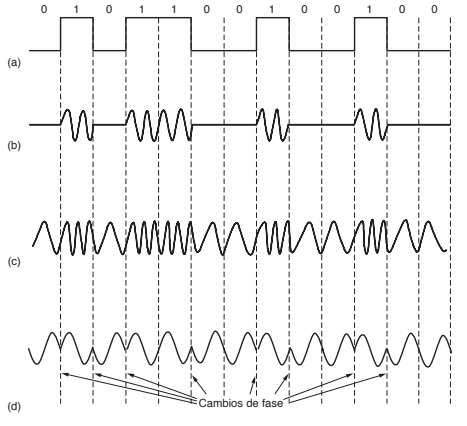
\includegraphics[width=0.65\linewidth]{IN1/IN25.png}
\caption{a. Señal binaria b. ASK c. FSK d. PSK}
\label{fig: modulacion ancho B}
\end{figure}
Se pueden mezclar estas modulaciones para obtener más símbolos enviados pero solo se puede modular o bien frecuencia o bien fase, nunca ambos,. ya que están relacionadas; la frecuencia es la tasa de cambio de la fase a través del tiempo. La más común es combinar amplitud con fase, en esta combinación es común representarlas como \textbf{diagramas de constelación} y suelen usar el término \textbf{QAM} (Modulación por amplitud de cuadratura) (Fig. \ref{fig: diagrama de constelación}), a más puntos en los diagramas se puede transmitir más bits por símbolo, es decir con una modulación QAM-64 se pueden transmitir 6 bits por símbolo. Las modulaciones y los bits por símbolo estas relacionados por potencias de 2.\\
Es de vital importancia que receptor pueda ubicar correctamente el inicio del tren de símbolos: si enviamos por ejemplo 0101-1011; si el receptor lee mal (ruido) puede leer 1011-0110 y toda la información estaría errónea. Por eso se utiliza \textbf{código Gray}, donde la diferencia entre los símbolos es solo de un bit. (Fig. \ref{fig: qam gray}), el error solo es de un bit, y no es tan drástico como lo sería una codificación binaria simple.
\begin{figure}[]
\centering
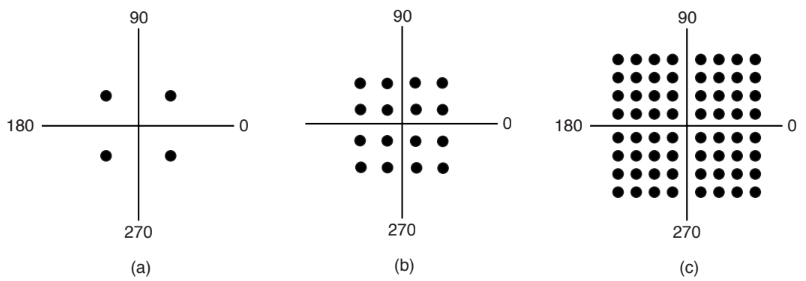
\includegraphics[width=\linewidth]{IN1/IN26.png}
\caption{a. QPSK b. QAM-16 c. QAM-64}
\label{fig: diagrama de constelación}
\end{figure}
\begin{figure}[]
\centering
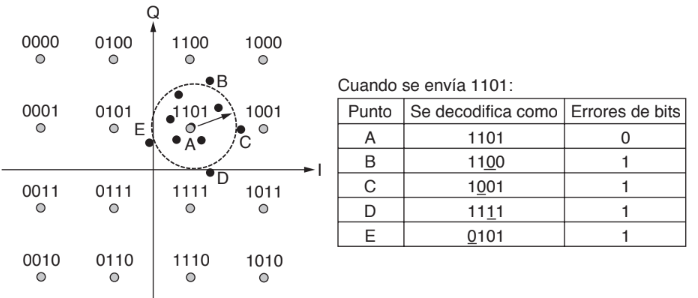
\includegraphics[width=\linewidth]{IN1/IN27.png}
\caption{QAM-16 con código Gray}
\label{fig: qam gray}
\end{figure}
En la imagen \ref{fig: qam gray} se notan los posibles resultados de una decodificación alterada por el ruido y sus posibles lecturas donde solo difieren en un bit.
\section{Multiplexión por división de frecuencia-FDM}\index{Multiplexión por división de frecuencia-FDM}
Aprovecha la transmisión pasa-banda, el ejemplo más claro es la radio: donde para la modulación AM se divide el ancho de banda dedicado a la radio AM en sub-bandas, y cada sub-banda o canal lógico sería cada estación de radio. En la Fig. \ref{fig: fdm mul} se muestra en Fig. \ref{fig: fdm mul}.a 3 servicios de telefonía, cada uno entro de las frecuencias útiles del caso (para telefonía es de 3100 KHz). Luego cada una de las sub-bandas se elevan en frecuencia (Fig. \ref{fig: fdm mul}.b) en distintos factores pues no deben compartir la misma frecuencia, si existe un espacio vacío entre ambas sub-bandas, a ese espacio se le llama \textbf{banda de guarda}; una vez que estén elevadas en frecuencias se pueden transmitir en el espectro electromagnético (Fig. \ref{fig: fdm mul}.c). Notesé que en las fronteras de cada sub-banda existe un cruce porque los filtros que la controlan no son ideales, es decir no cortan en seco, sino hay un desvanecimiento.
\begin{figure}[]
\centering
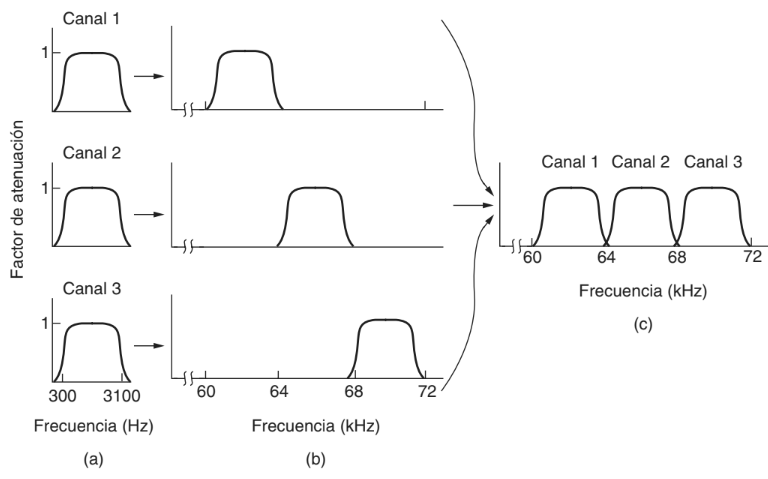
\includegraphics[width=0.7\linewidth]{IN1/IN28.png}
\caption{a. Anchos de banda originales b. Anchos de banda elevados en frecuencia c. Canal multiplexado}
\label{fig: fdm mul}
\end{figure}
\section{Multiplexión por división de tiempo-TDM}
Alternativa el TDM, aquí cada usuario ocupa todo el ancho de banda durante un periodo pequeño de tiempo, y pasa al siguiente usuario (Fig. \ref{fig: tdm}). Se tomán bits de cada entrada en una sola \textbf{ranura de tiempo}, este flujo opera a una velocidad de la suma de los flujos individuales. NO confundir con \textbf{STDM}.
\begin{figure}[H]
\centering
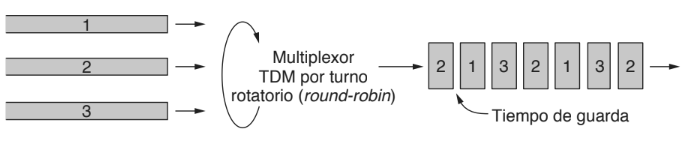
\includegraphics[width=\linewidth]{IN1/IN29.png}
\caption{Multiplexación por división de tiempo.}
\label{fig: tdm}
\end{figure}
4 conexiones T1 a 1.554Mbps, multiplexadas por TDM originan una conexión T2 a 6.312 Mbps, 7 conexiones T2 por TDM originan una conexión T3 a 44.736 Mbps y por último 6 T3 en TDM generan una conexión T4 a 274.176 Mbps. (Fig. \ref{fig: t1 carrier})
\begin{figure}[]
\centering
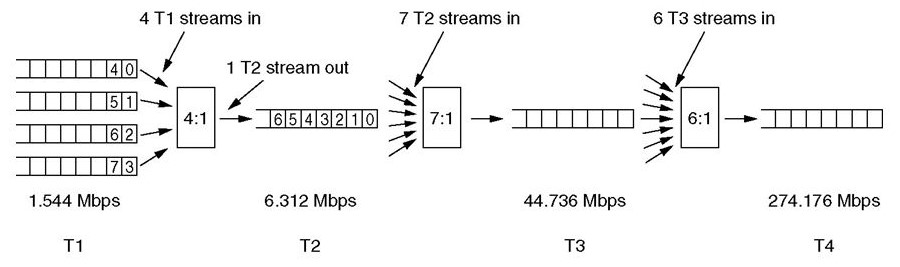
\includegraphics[width=0.7\linewidth]{IN1/IN30.png}
\caption{Multiplexación de una portadora T1 en portadoras mayores.}
\label{fig: t1 carrier}
\end{figure}
%\section{Capa de enlace y la evolución de las telecomunicaciones}
%----------------------------------------------------------------------------------------
%Microprocesadores
%----------------------------------------------------------------------------------------

%----------------------------------------------------------------------------------------
%Mantenimiento
%----------------------------------------------------------------------------------------
%21:27 falta material
%----------------------------------------------------------------------------------------
\end{document}
%----------------------------------------------------------------------------------------
